\chapter{Materials and methods}
Medical images such as CT scans of brain are collected from the archives of hospitals that routinely screen patients for cancer. Around 180 cases are used for the work.
\section{Preprocessing and segmentation}

Here, we only briefly describe the preprocessing and segmentation methods of the proposed CAD system \cite{einstein}. Image enhancement is one of the most important issues in low-level image processing. The underlying principle of the enhancement is to enlarge the intensity difference between objects and surroundings without both the over enhancement and under enhancement. A lot of enhancement methods have been developed that can mainly be divided into two classes: local and global methods. We employ the previously developed Multi-peak GHE (Generalized Histogram Equalization) method due to its effectiveness in enhancing the image and its textures. By changing the order of the gray levels in the image, the enhancement procedure is made completely controllable. Image segmentation can be considered as a labelling problem wherein the solution is to assign a set of labels to image pixels. The algorithm based on Markov Random Field (MRF) is adopted in this paper. It makes the system more consistent with the global model. Therefore, it is more tolerant to noise, and requires less iteration to converge \cite{latexcompanion}.

\begin{figure}[h]
\centering
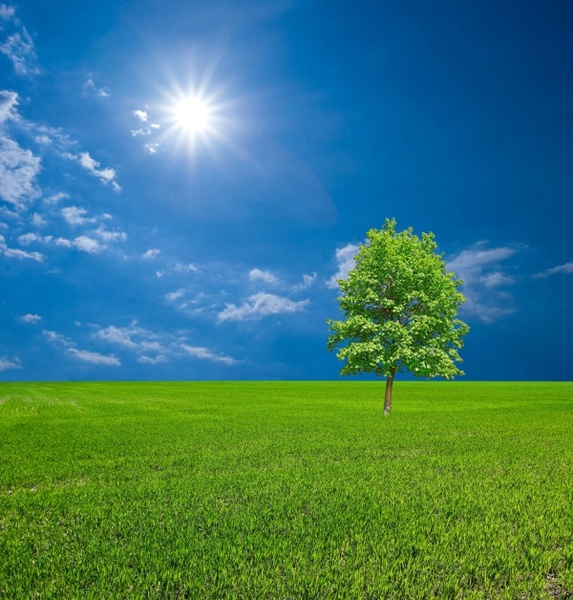
\includegraphics[width=8cm]{chapters/1.jpg}
\caption{An example graph}
\label{graph}
\end{figure}





 shows the flowchart of the proposed approach. Fig \ref{graph} show the original image and its multi-peak histogram equalized image.
    
\section{ Feature extraction and selection} 

A key stage of tumour detection and classification by Computer-Aided Diagnosis (CAD) schemes is feature analysis and extraction. The most important issue in feature analysis is that the selected features should be able to represent the characteristics of the tumours, and based on these features, the malignant can be discriminated from the benign ones.
\subsection {Textural features}
Textural features are based on co-occurrence matrices of the texture information. All textural features are derived 
\begin{figure}[h]
\centering
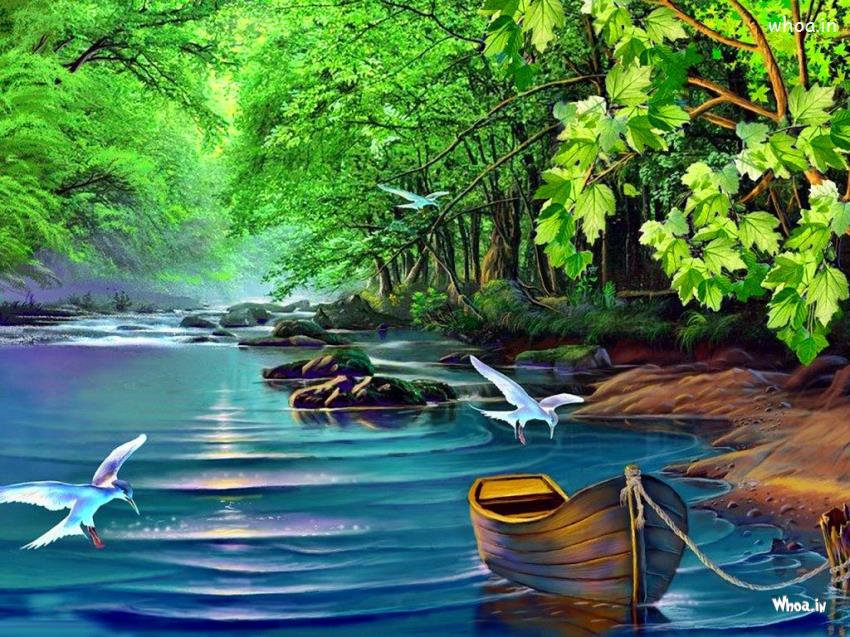
\includegraphics[width=8cm]{chapters/river.jpg}
\caption{river}
\label{river}
\end{figure}

